% Provenance (never printed): see sources/outline_sources.md (Year 3:
% planetary atmospheres, escape, the runaway greenhouse, Mars, Titan,
% habitability).
% Brief: sources/book5/BRIEFS.md, ch. 27. Curves from figdata/bachelor-3/
% jeans_escape.py (escape parameter and escaping fraction at the exobases
% of Venus, the Earth, Mars and Titan), runaway_greenhouse.py (an
% illustrative grey model of a moist atmosphere: OLR against surface
% temperature) and habitability.py (the habitable-zone fits of Kopparapu et
% al. 2013; the phase boundaries of water and methane with the surface
% states of four bodies). Exercise and problem values in the Book 5 scratch
% calculator calc/ch27.py. Kepos and its star are invented.
\chapter{Atmosphères planétaires et habitabilité}\label{ch:b3:planetary-atmospheres}

Vénus et la Terre sont presque des jumelles~: quasiment la même taille, des
masses volumiques moyennes voisines, des orbites voisines. Pourtant Vénus conserve \qty{92}{bar} de dioxyde de carbone
au-dessus d'une surface à \qty{737}{K}, et si peu d'eau que, étalée
sur sa surface, elle formerait une couche d'à peine un centimètre d'épaisseur. Le spectromètre de masse
de la sonde Pioneer Venus, en traversant ses nuages, a mesuré le rapport du
deutérium à l'hydrogène dans cette eau~: \num{0.016}, soit cent fois le
rapport observé dans les océans terrestres. L'hydrogène léger s'échappe dans
l'espace plus facilement que le deutérium lourd~; ce qui reste d'un grand réservoir
ayant perdu l'essentiel de son hydrogène s'enrichit en deutérium. Ce rapport est la
trace de l'eau que Vénus a possédée, puis perdue. Ce chapitre se demande comment une
planète retient son air et son eau, et comment elle les perd.
% ledger: planet:Venus.diameter, planet:Earth.diameter, planet:Venus.density, planet:Earth.density, nasa:venus-atm, arney18:venus-water, donahue82:dh, kc98:standards

\begin{recall}
La hauteur d'échelle, la formule barométrique, la distribution de
Maxwell--Boltzmann, la vitesse de libération, le libre parcours moyen et l'effet
de serre sont dans les volumes de physique. La zone habitable d'une étoile figure
dans les manuels du secondaire. La température d'équilibre et l'albédo de Bond sont
dans le volume de première année, dans son chapitre de planétologie comparée~; la
profondeur optique, dans son chapitre sur les télescopes et la photométrie~; les
gradients de température, dans son chapitre sur la structure de l'atmosphère et de
l'océan~; le rayonnement infrarouge sortant (OLR) et la température d'émission, dans
son chapitre sur le rayonnement et le transport de chaleur. L'adiabatique humide est
dans le volume de deuxième année, dans son chapitre sur la thermodynamique
atmosphérique~; la ligne des glaces, dans son chapitre sur la formation planétaire~; le
cycle long du carbone et le thermostat de l'altération des silicates, dans son chapitre
sur le climat aux échelles géologiques. La \omterm{prop:b3:stable-isotopes:rayleigh-distillation}{distillation de Rayleigh} est dans ce volume,
dans son chapitre sur les isotopes stables.
\end{recall}

\section{La structure d'une atmosphère}\label{sec:b3:planetary-atmospheres:structure}

Une atmosphère isotherme de masse moléculaire $m$ à la température $T$ s'amincit
avec l'altitude selon $p = p_0\,e^{-z/H}$, avec la hauteur d'échelle $H = kT/mg$.
À la surface de la Terre, $H$ vaut environ \qty{8}{km}~; à la surface de
Titan, où la pesanteur est faible et l'air froid, environ \qty{20}{km}.

La température, cependant, n'est pas uniforme. Le rayonnement solaire qui
atteint le sol le réchauffe~; l'air situé au-dessus, qui absorbe et émet
dans l'infrarouge, est réchauffé par le bas. Le seul rayonnement rendrait la
basse atmosphère si raide en température qu'elle se renverserait.

\begin{definition}[Équilibre radiatif--convectif]\label{def:b3:planetary-atmospheres:rce}
Une colonne d'atmosphère est en \emph{équilibre
radiatif--convectif}\index{equilibre radiatif--convectif@équilibre radiatif--convectif} lorsque, à chaque niveau, le flux net de rayonnement
est équilibré, sauf dans une couche inférieure où la convection transporte la
chaleur vers le haut et maintient le gradient de température à la valeur
adiabatique. La couche inférieure, convective, est la troposphère~; la couche
supérieure, en équilibre radiatif, est la stratosphère~; la tropopause est le
niveau où elles se rejoignent.
\end{definition}

L'atmosphère la plus simple sur laquelle on peut suivre ce raisonnement est \emph{grise}~: elle
est transparente au rayonnement solaire et absorbe toutes les longueurs d'onde infrarouges de la même façon,
avec une profondeur optique $\tau$ comptée vers le bas à partir du sommet.

\begin{proposition}[Équilibre radiatif gris]\label{prop:b3:planetary-atmospheres:grey}
Dans une atmosphère grise en équilibre radiatif qui émet le flux $F$ vers
l'espace, la température à la profondeur optique $\tau$ obéit à
\[
\sigma T^4(\tau) = \frac F2\,(1 + D\tau),
\]
où $D \approx 1.66$ rend compte des trajets obliques du rayonnement.
Le sommet de l'atmosphère se trouve à la \emph{température de peau}
$T_\mathrm{skin} = 2^{-1/4}\,T_e$, où $T_e = (F/\sigma)^{1/4}$ est la
température d'émission.
\end{proposition}

La proposition est admise~; elle découle des équations à deux flux pour les
flux montant et descendant. Là où $\tau$ est grand, près du sol, la
température radiative varie vite avec $\tau$, et $\tau$ lui-même croît
rapidement avec la profondeur parce que le gaz absorbant est le plus dense
là~: le profil radiatif est plus raide que l'adiabate, et la convection prend
le relais. En altitude, $\tau$ est petit et la température tend vers la
température de peau. La Terre émet environ \qty{239}{W.m^{-2}} vers l'espace,
avec une température d'émission de \qty{255}{K} et une température de peau de
\qty{214}{K}~; l'atmosphère standard place sa tropopause à \qty{11}{km}
et à \qty{216.65}{K}. Le modèle gris, pour sommaire qu'il soit, situe à peu près
bien le sommet froid de la troposphère.
% ledger: ipcc:budget-toa, ussa76:sea-level, ussa76:layers, const:sigma

\begin{omfigure}
\centering
\begin{tikzpicture}[x=1cm, y=0.8cm, font=\small]
% temperature profile (schematic)
\draw[->] (0,0) -- (6.8,0) node[below left, font=\scriptsize] {température};
\draw[->] (0,0) -- (0,8.4) node[above, font=\scriptsize] {altitude};
\draw[thick, omDef] (5.6,0) -- (4.2,2.0) -- (4.2,2.6) -- (4.7,3.6)
  -- (3.8,4.6) .. controls (4.3,5.6) and (5.9,6.0) .. (6.2,6.6) -- (6.25,8.2);
\draw[dashed, black!50] (0,2.0) -- (6.8,2.0) node[right, font=\scriptsize, black] {tropopause};
\draw[dashed, black!50] (0,4.6) -- (6.8,4.6) node[right, font=\scriptsize, black] {homopause};
\draw[thick, red!70!black] (0,6.6) -- (6.8,6.6) node[right, font=\scriptsize] {exobase};
\node[anchor=west, font=\scriptsize] at (0.15,0.9) {troposphère~: convection};
\node[anchor=west, font=\scriptsize] at (0.15,0.5) {(adiabate)};
\node[anchor=west, font=\scriptsize] at (0.15,3.2) {stratosphère~:};
\node[anchor=west, font=\scriptsize] at (0.15,2.8) {équilibre radiatif};
\node[anchor=west, font=\scriptsize] at (0.15,5.6) {thermosphère};
\node[anchor=west, font=\scriptsize] at (0.15,5.2) {(chauffée par l'EUV)};
\node[anchor=west, font=\scriptsize] at (0.15,7.6) {exosphère~:};
\node[anchor=west, font=\scriptsize] at (0.15,7.2) {sans collisions};
% exosphere trajectories
\begin{scope}[shift={(11.0,0)}]
\fill[black!8] (-2.3,0) rectangle (2.3,6.6);
\draw[red!70!black, thick] (-2.3,6.6) -- (2.3,6.6);
\node[font=\scriptsize] at (0,0.5) {collisions partout};
\node[font=\scriptsize, align=center] at (0,3.3) {gaz mélangé par\\la turbulence\\sous l'homopause,\\séparé par diffusion\\moléculaire au-dessus};
\draw[->, thick, omDef] (-1.6,6.6) .. controls (-1.4,8.0) and (-0.9,8.0) .. (-0.7,6.6);
\node[font=\scriptsize, omDef] at (-1.15,8.3) {balistique};
\draw[->, thick, red!70!black] (0.4,6.6) -- (1.2,8.5);
\node[font=\scriptsize, red!70!black, anchor=west] at (1.25,8.3) {échappée};
\node[font=\scriptsize, align=center, anchor=north] at (0,6.45) {$v > v_\mathrm{esc}$ vers le haut~:\\ perdue dans l'espace};
\end{scope}
\end{tikzpicture}
\par\smallskip{\small Les couches d'une atmosphère planétaire (schéma, non à
l'échelle). À gauche~: un profil de température semblable à celui de la Terre, avec
la troposphère maintenue sur l'adiabate par la convection, une stratosphère en
équilibre radiatif et une thermosphère chauffée par le haut par le rayonnement
ultraviolet extrême du Soleil. À droite~: au-dessus de l'\omterm{def:b3:planetary-atmospheres:exobase}{exobase}, une particule
ne rencontre rien~; celle qui monte plus vite que la vitesse de libération quitte la
planète, celle qui est plus lente retombe sur une trajectoire balistique.}\label{fig:b3:planetary-atmospheres:structure}
\end{omfigure}
% ledger: gronoff:exobase, gronoff:diffusion

Très haut dans l'atmosphère, l'air est si ténu qu'une molécule peut parcourir une grande distance
entre deux collisions. Là où elle peut parcourir plus d'une hauteur d'échelle, elle n'appartient
plus à un fluide.

\begin{definition}[Exobase~; exosphère]\label{def:b3:planetary-atmospheres:exobase}
L'\emph{exobase}\index{exobase} d'une atmosphère est le niveau auquel le libre parcours moyen
de ses particules égale la hauteur d'échelle. Au-dessus,
dans l'\emph{exosphère}\index{exosphère}, une particule qui se déplace vers le haut
a peu de chances d'en rencontrer une autre, et une particule plus rapide que la vitesse
de libération locale quitte la planète.
\end{definition}

\begin{proposition}[Condition à l'exobase]\label{prop:b3:planetary-atmospheres:exobase}
Dans une atmosphère isotherme de particules de section efficace de collision
$\sigma_c$, une particule qui se déplace verticalement vers le haut depuis le niveau de densité
$n$ échappe à toute collision avec la probabilité $e^{-n\sigma_c H}$. À
l'\omterm{def:b3:planetary-atmospheres:exobase}{exobase} $n\sigma_c H = 1$~: la probabilité vaut $1/e$.
\end{proposition}

\begin{proof}
Le long d'un trajet $\mathrm dz$, la particule rencontre en moyenne $n(z)\sigma_c\,
\mathrm dz$ autres particules. La probabilité de n'en rencontrer aucune sur le trajet vers le haut depuis
$z_0$ vaut $\exp(-\sigma_c\int_{z_0}^\infty n\,\mathrm dz)$, et, dans une atmosphère
isotherme, $\int_{z_0}^\infty n_0\,e^{-(z-z_0)/H}\,\mathrm dz
= n_0 H$. Le libre parcours moyen vaut $\ell = 1/n\sigma_c$~; la condition $\ell
= H$ s'écrit $n\sigma_c H = 1$.
\end{proof}

L'\omterm{def:b3:planetary-atmospheres:exobase}{exobase} se situe à environ \qty{500}{km} sur la Terre, à \qty{200}{km}
sur Vénus et sur Mars, et vers \qty{1500}{km} sur Titan, soit plus de la moitié du
rayon de la lune.
% ledger: gronoff:exobases

\section{Échappement atmosphérique}\label{sec:b3:planetary-atmospheres:escape}

À l'\omterm{def:b3:planetary-atmospheres:exobase}{exobase}, les particules conservent la distribution de Maxwell--Boltzmann
des vitesses du gaz situé en dessous. La queue de cette distribution contient toujours quelques particules plus rapides
que la vitesse de libération.

\begin{definition}[Échappement de Jeans~; paramètre d'échappement]\label{def:b3:planetary-atmospheres:jeans-escape}
L'\emph{échappement de Jeans}\index{echappement de Jeans@échappement de Jeans} est la perte vers l'espace des
particules de la queue de Maxwell--Boltzmann qui se déplacent vers le haut à l'\omterm{def:b3:planetary-atmospheres:exobase}{exobase}
à une vitesse supérieure à la vitesse de libération. Le \emph{paramètre
d'échappement}\index{paramètre d'échappement} des particules de masse $m$ à l'\omterm{def:b3:planetary-atmospheres:exobase}{exobase},
de rayon $r$ et de température $T$, sur une planète de masse $M$, vaut
\[
\lambda = \frac{GMm}{kTr} = \frac{v_\mathrm{esc}^2}{u^2},
\qquad u = \sqrt{\frac{2kT}m},
\]
c'est le rapport de leur énergie de liaison gravitationnelle à $kT$, et aussi le carré
de la vitesse de libération divisée par la vitesse thermique la plus probable $u$.
\end{definition}

\begin{theorem}[Flux de Jeans]\label{thm:b3:planetary-atmospheres:jeans}
À un \omterm{def:b3:planetary-atmospheres:exobase}{exobase} de densité $n$, le nombre de particules qui s'échappent par unité
de surface et par unité de temps vaut
\[
\Phi_\mathrm J = \frac{n\,u}{2\sqrt\pi}\,(1 + \lambda)\,e^{-\lambda}.
\]
\end{theorem}

\begin{proof}
La distribution de Maxwell--Boltzmann des vitesses est $f(\vec v) =
n\,(\pi u^2)^{-3/2}\,e^{-v^2/u^2}$. Une particule de vitesse $v$ faisant un angle
$\theta$ avec la verticale traverse une aire horizontale unité au
rythme $v\cos\theta$. En ne comptant que les vitesses dirigées vers le haut ($0 \le \theta \le
\pi/2$) supérieures à $v_\mathrm{esc}$,
\[
\Phi_\mathrm J = \frac{n}{\pi^{3/2}u^3}\int_0^{2\pi}\!\!\mathrm d\varphi
\int_0^{\pi/2}\!\!\cos\theta\sin\theta\,\mathrm d\theta
\int_{v_\mathrm{esc}}^\infty v^3e^{-v^2/u^2}\,\mathrm dv
= \frac{n}{\pi^{3/2}u^3}\cdot2\pi\cdot\frac12\cdot
\frac{u^4}2\,(1 + \lambda)\,e^{-\lambda},
\]
où la dernière intégrale résulte du changement de variable $s = v^2/u^2$ et d'une
intégration par parties~: $\int_\lambda^\infty s\,e^{-s}\,\mathrm ds =
(1 + \lambda)e^{-\lambda}$. En regroupant, $\Phi_\mathrm J = n u (1 +
\lambda) e^{-\lambda}/(2\sqrt\pi)$.
\end{proof}

Le facteur $n u/2\sqrt\pi$ est le flux de toutes les particules qui traversent
l'\omterm{def:b3:planetary-atmospheres:exobase}{exobase} vers le haut~; $(1 + \lambda)e^{-\lambda}$ est la fraction d'entre elles
qui s'échappent. Elle décroît exponentiellement avec la masse de la particule, puisque
$\lambda \propto m$. À l'\omterm{def:b3:planetary-atmospheres:exobase}{exobase} terrestre, à \qty{1000}{K}, l'hydrogène
a $\lambda = 7.0$ et s'échappe à un taux de 0.7\,\% de son flux
ascendant~; le deutérium, $\lambda = 14$, à \num{1.2e-5}~; l'hélium, $\lambda = 28$,
à \num{2e-11}~; l'oxygène, $\lambda = 111$, pas du tout. À l'\omterm{def:b3:planetary-atmospheres:exobase}{exobase} de
Vénus, plus froide et tout aussi profonde dans le puits de gravité, $\lambda = 22$ même pour
l'hydrogène~; sur Mars, $\lambda = 5.4$~; sur Titan, $\lambda = 1.5$ pour l'hydrogène
et 3.0 pour le dihydrogène.
% ledger: gronoff:jeans, gronoff:jeans-table, gronoff:exobases

\begin{omfigure}
\centering
\begin{tikzpicture}
\begin{axis}[name=lam, width=0.47\linewidth, height=0.46\linewidth,
  xmin=0.5, xmax=50, ymin=0.5, ymax=2000, xmode=log, ymode=log,
  xlabel={masse de la particule (u)}, ylabel={paramètre d'échappement $\lambda$},
  tick label style={font=\scriptsize}, label style={font=\small},
  xtick={1,2,4,16,28,44}, xticklabels={1,2,4,16,28,44},
  title={(a)}, title style={font=\small},
  legend style={font=\scriptsize, at={(0.5,-0.24)}, anchor=north, legend columns=2, draw=none}]
\fill[black!10] (axis cs:0.5,0.5) rectangle (axis cs:50,2.5);
\node[font=\scriptsize, anchor=east] at (axis cs:40,1.0) {hydrodynamique};
\addplot[thick, orange!80!black] table[x=A, y=Venus] {figdata/out/bachelor-3-jeans_escape-lambda.dat};
\addlegendentry{Vénus}
\addplot[thick, omDef] table[x=A, y=Earth] {figdata/out/bachelor-3-jeans_escape-lambda.dat};
\addlegendentry{Terre}
\addplot[thin, omDef, dashed, forget plot] table[x=A, y=EarthLo] {figdata/out/bachelor-3-jeans_escape-lambda.dat};
\addplot[thin, omDef, dashed, forget plot] table[x=A, y=EarthHi] {figdata/out/bachelor-3-jeans_escape-lambda.dat};
\addplot[thick, red!70!black] table[x=A, y=Mars] {figdata/out/bachelor-3-jeans_escape-lambda.dat};
\addlegendentry{Mars}
\addplot[thick, black!60] table[x=A, y=Titan] {figdata/out/bachelor-3-jeans_escape-lambda.dat};
\addlegendentry{Titan}
\end{axis}
\begin{axis}[at={(lam.east)}, anchor=west, xshift=0.1\linewidth,
  width=0.47\linewidth, height=0.46\linewidth,
  xmin=0, xmax=40, ymin=1e-16, ymax=1, ymode=log,
  xlabel={paramètre d'échappement $\lambda$}, ylabel={fraction échappée},
  ytick={1e-16,1e-12,1e-8,1e-4,1},
  tick label style={font=\scriptsize}, label style={font=\small},
  title={(b)}, title style={font=\small}]
\addplot[thick, black] table[x=lam, y=f] {figdata/out/bachelor-3-jeans_escape-factor.dat};
\addplot[only marks, mark=*, mark size=1.8pt, omDef] table[x=lambdaEarth, y=fEarth] {figdata/out/bachelor-3-jeans_escape-species.dat};
\node[font=\scriptsize, omDef, anchor=south west] at (axis cs:7.0,7.1e-3) {H};
\node[font=\scriptsize, omDef, anchor=south west] at (axis cs:14.0,1.2e-5) {D};
\node[font=\scriptsize, omDef, anchor=south west] at (axis cs:27.9,2.2e-11) {He};
\end{axis}
\end{tikzpicture}
\par\smallskip{\small (a)~Le \omterm{def:b3:planetary-atmospheres:jeans-escape}{paramètre d'échappement} à l'\omterm{def:b3:planetary-atmospheres:exobase}{exobase} en fonction de la
masse de la particule, pour Vénus (\qty{290}{K}), la Terre (\qty{1000}{K}~;
en pointillés~: 800 et \qty{1600}{K}, l'amplitude du cycle solaire), Mars
(\qty{270}{K}) et Titan (\qty{180}{K})~; en dessous de $\lambda \approx 2.5$
(zone grisée), l'échappement devient hydrodynamique. (b)~La fraction $(1 +
\lambda)e^{-\lambda}$ du flux ascendant qui s'échappe, avec l'hydrogène,
le deutérium et l'hélium à l'\omterm{def:b3:planetary-atmospheres:exobase}{exobase} terrestre~; l'oxygène, à $\lambda = 111$,
se trouve hors de l'échelle.}\label{fig:b3:planetary-atmospheres:jeans}
\end{omfigure}
% ledger: gronoff:jeans-table, gronoff:exobases, gronoff:jeans, nasa:venus, planet:Earth.mass, nasa:mars, nasa:titan, const:G, const:kB

Lorsque $\lambda$ descend à quelques unités, l'image de particules qui s'échappent une à une
d'une atmosphère statique ne tient plus~: la haute atmosphère se dilate et s'écoule
vers l'espace comme un vent. Les modèles placent la transition à $\lambda$ compris entre environ 1.5
et 3.

\begin{definition}[Échappement hydrodynamique, non thermique et limité par la diffusion]\label{def:b3:planetary-atmospheres:hydrodynamic}
L'\emph{échappement hydrodynamique}\index{echappement@échappement hydrodynamique} est la perte d'une
haute atmosphère qui s'écoule en bloc, chauffée par le haut, lorsque son \omterm{def:b3:planetary-atmospheres:jeans-escape}{paramètre
d'échappement} est petit~; l'écoulement peut entraîner avec lui des particules plus lourdes.
L'\emph{échappement non thermique}\index{echappement@échappement non thermique} est la perte
de particules accélérées par des processus autres que la chaleur~: réactions
photochimiques qui donnent aux fragments plus que l'énergie d'échappement, ions captés
par le champ électrique du vent solaire, pulvérisation par des ions qui frappent
la haute atmosphère, et écoulement d'ions le long des lignes du champ magnétique.
L'\emph{échappement limité par la diffusion}\index{echappement@échappement limité par la diffusion} est un échappement
dont le débit n'est pas fixé à l'\omterm{def:b3:planetary-atmospheres:exobase}{exobase} mais plus bas, par la vitesse à laquelle le gaz
qui s'échappe peut diffuser vers le haut à travers le gaz plus lourd situé au-dessus de
l'\emph{homopause}\index{homopause}, niveau au-dessus duquel la diffusion moléculaire, et non la turbulence,
commande le mélange.
\end{definition}
% ledger: gronoff:jeans, gronoff:nonthermal, gronoff:diffusion

\begin{proposition}[Limite de diffusion]\label{prop:b3:planetary-atmospheres:diffusion}
Un gaz léger de rapport de mélange $f$ et de masse moléculaire $m_i$, diffusant
à travers un gaz plus lourd de masse moléculaire $m_a$ et de hauteur d'échelle $H_a =
kT/m_a g$ avec le paramètre de diffusion binaire $b$, ne peut pas monter plus vite
que
\[
\Phi_\mathrm{DL} = b\,f\left(\frac1{H_a} - \frac1{H_i}\right)
= \frac{b\,f\,(m_a - m_i)\,g}{kT} \approx \frac{b\,f}{H_a}.
\]
\end{proposition}

\begin{proof}
La théorie cinétique (admise) donne le flux ascendant du gaz léger
par rapport au gaz lourd, dans une colonne isotherme, sous la forme $\Phi = -b\,f\,
[\,(1/f)\,\mathrm df/\mathrm dz + 1/H_i - 1/H_a\,]$~: le gaz léger diffuse vers le bas le long de son propre gradient, et sa
hauteur d'échelle propre $H_i$ est plus grande que $H_a$. Le flux est maximal lorsque le
rapport de mélange est uniforme, $\mathrm
df/\mathrm dz = 0$~: le gaz qui s'échappe ne peut pas être extrait plus vite sans que son
rapport de mélange ne diminue avec l'altitude. Avec $1/H = mg/kT$, les deux formes
se déduisent l'une de l'autre.
\end{proof}

Pour l'hydrogène moléculaire qui monte à travers le dioxyde de carbone, $b \approx
\qty{1.2e19}{cm^{-1}.s^{-1}}$ à \qty{200}{K}, et avec la pesanteur terrestre
la limite vaut $\Phi_\mathrm{DL} \approx
\num{3.0e13}\,f\,(\qty{200}{K}/T)^{1/4}$ molécules de $\ce{H2}$ par
centimètre carré et par seconde, $f$ comptant tout l'hydrogène comme $\ce{H2}$. Sur
la Terre actuelle, l'échappement de l'hydrogène est limité par la diffusion~: au minimum solaire,
lorsque l'\omterm{def:b3:planetary-atmospheres:exobase}{exobase} est plus froide et que l'\omterm{def:b3:planetary-atmospheres:jeans-escape}{échappement de Jeans} est plus lent, l'échappement
par échange de charge avec les ions prend le relais, et le total reste à peu près
le même. L'apport, et non
l'\omterm{def:b3:planetary-atmospheres:exobase}{exobase}, fixe le débit.
% ledger: zahnle19:diffusion, gronoff:diffusion, gronoff:rates

\section{Vénus et l'effet de serre galopant}\label{sec:b3:planetary-atmospheres:venus}

Vénus reçoit \qty{2601}{W.m^{-2}} du Soleil, soit 1.91 fois la part
de la Terre. Ses nuages d'acide sulfurique en réfléchissent 77\,\%, de sorte qu'elle absorbe
moins que la Terre~; pourtant sa surface est à \qty{737}{K} sous \qty{92}{bar}
d'une atmosphère composée à 96.5\,\% de dioxyde de carbone. Elle contient \qty{6e15}{kg} d'eau,
contre \qty{1.4e21}{kg} sur la Terre, soit environ 30 parties par million en volume
sous les nuages.
% ledger: nasa:venus, nasa:venus-atm, arney18:venus-water

Une planète dotée d'un océan est maintenue en équilibre par son rayonnement sortant. Si
elle se réchauffe, davantage d'eau s'évapore~; la vapeur d'eau est un gaz à effet de serre, de sorte que le
rayonnement sortant croît moins vite que $\sigma T^4$, mais il croît, et le
réchauffement s'arrête. Cette croissance a une limite.

\begin{proposition}[Limite par rayonnement d'une atmosphère humide]\label{prop:b3:planetary-atmospheres:limit}
Lorsque la surface d'une planète océanique est assez chaude pour que la vapeur d'eau
domine sa haute atmosphère, la température y suit la
courbe de saturation de l'eau, et le rayonnement infrarouge vers l'espace provient
d'un niveau de pression fixe. Sa température, et le rayonnement sortant,
cessent de croître avec la température de surface.
\end{proposition}

\begin{proof}
Dans une colonne saturée dominée par la vapeur, la pression $p$ à chaque
niveau est la pression de saturation à la température locale, $p =
p_\mathrm{sat}(T)$. Le rayonnement vers l'espace part des alentours du niveau
où la profondeur optique depuis le sommet vaut environ un. Pour un gaz gris de
coefficient d'absorption massique $\kappa$, la profondeur optique au-dessus de la pression $p$
vaut $D\kappa p/g$, de sorte que ce niveau se situe en $p_1 = g/D\kappa$, quelle que soit la
température de surface, et sa température est celle pour laquelle
$p_\mathrm{sat}(T) = p_1$. Réchauffer la surface ne fait qu'ajouter de la vapeur en dessous.
\end{proof}

\begin{definition}[Effet de serre galopant~; limite de l'effet de serre galopant~; effet de serre humide]\label{def:b3:planetary-atmospheres:runaway}
La \emph{limite de l'effet de serre galopant}\index{limite de l'effet de serre galopant} est le
flux de rayonnement infrarouge le plus élevé qu'une planète dotée d'un océan puisse envoyer vers
l'espace. Un \emph{effet de serre galopant}\index{effet de serre galopant} est l'état
d'une planète qui absorbe plus de lumière solaire que cette limite~: elle ne peut pas équilibrer son
bilan avant que tout l'océan ne se soit évaporé et que la surface ne se soit
échauffée bien au-delà. Un \emph{effet de serre humide}\index{effet de serre humide}
est l'état d'une planète, en deçà de l'emballement, dont la surface est assez chaude
pour que sa stratosphère contienne un rapport de mélange élevé de vapeur d'eau,
que le rayonnement ultraviolet dissocie et dont l'hydrogène s'échappe.
\end{definition}

Des modèles simples, comme celui de la proposition, donnent une telle limite~; avec les
raies réelles de la vapeur d'eau, un calcul raie par raie sans nuages
la place à \qty{291}{W.m^{-2}} pour une planète de type terrestre, et
les revues en donnent environ \qty{300}{W.m^{-2}}. Au-delà d'environ \qty{2000}{K}, le
flux sortant augmente à nouveau, car la basse atmosphère chaude rayonne dans le
visible et le proche infrarouge, où l'eau absorbe peu~: une planète en
\omterm{def:b3:planetary-atmospheres:runaway}{effet de serre galopant} se stabilise à une température très élevée, une fois que son océan
est entièrement passé à l'état de vapeur.
% ledger: kopparapu13:runaway, arney18:runaway

\begin{omfigure}
\centering
\begin{tikzpicture}
\begin{axis}[width=0.8\linewidth, height=0.48\linewidth,
  xmin=250, xmax=600, ymin=150, ymax=560,
  xlabel={température de surface (\unit{K})},
  ylabel={flux (\unit{W.m^{-2}})},
  tick label style={font=\scriptsize}, label style={font=\small}]
\addplot[very thick, omDef] table[x=Ts, y=olr] {figdata/out/bachelor-3-runaway_greenhouse-olr.dat};
\addplot[dashed, black!60, domain=250:600] {291};
\addplot[thick, orange!80!black, domain=250:600] {525};
\addplot[thick, orange!60!black, densely dotted, domain=250:600] {367};
\addplot[thick, black!70, densely dashed, domain=250:600] {238};
\node[font=\scriptsize, black!60, anchor=south east] at (axis cs:595,291) {limite raie par raie, \qty{291}{W.m^{-2}}};
\node[font=\scriptsize, orange!80!black, anchor=south east] at (axis cs:595,525) {Vénus actuelle, sans nuages};
\node[font=\scriptsize, orange!60!black, anchor=south east] at (axis cs:595,367) {jeune Vénus, Soleil à 70\,\%};
\node[font=\scriptsize, black!70, anchor=north east] at (axis cs:595,236) {la Terre actuelle};
\node[font=\scriptsize, omDef, anchor=west] at (axis cs:264,212) {rayonnement sortant (modèle)};
\end{axis}
\end{tikzpicture}
\par\smallskip{\small Rayonnement infrarouge sortant d'une planète océanique de type terrestre
en fonction de sa température de surface, dans un modèle gris illustratif
(une adiabatique humide saturée sur \qty{1}{bar} d'azote, une stratosphère à
\qty{200}{K}, la vapeur d'eau comme seul absorbant~; son coefficient d'absorption,
élargi par la pression, est choisi pour atteindre la limite raie par raie).
Droites horizontales~: rayonnement solaire absorbé par Vénus actuelle et par une jeune Vénus
d'albédo 0.193, l'albédo d'une atmosphère chaude de vapeur sans nuages,
et par la Terre actuelle avec son albédo de 0.3. Lorsque le flux absorbé
se situe au-dessus du palier, aucune température de surface ne l'équilibre~: l'effet de serre
s'emballe.}\label{fig:b3:planetary-atmospheres:runaway}
\end{omfigure}
% ledger: kopparapu13:runaway, iapws:vapour-pressure, iapws4:sublimation, const:R, const:sigma, nasa:venus, gough81:luminosity, ipcc:budget-toa

Avec l'albédo d'une atmosphère de vapeur sans nuages, 0.193, une planète de type terrestre
autour du Soleil s'emballe lorsqu'elle reçoit 1.06 fois l'ensoleillement terrestre, à
\qty{0.97}{au}. Auparavant, à 1.015 fois l'ensoleillement terrestre et pour une température
de surface de \qty{340}{K}, sa stratosphère devient humide~: sur la Terre actuelle, l'eau
est piégée par le froid à la tropopause, vers \qty{0.1}{bar}, mais sur une planète plus
chaude le piège froid remonte et laisse passer la vapeur. Lorsque le rapport de mélange
de l'eau dans la stratosphère atteint environ \num{3e-3}, l'\omterm{def:b3:planetary-atmospheres:hydrodynamic}{échappement limité
par la diffusion} retire un océan d'hydrogène en un temps voisin de
l'âge de la Terre.
% ledger: kopparapu13:runaway, kopparapu13:water-loss, arney18:runaway

Le deutérium de Vénus mesure ce qui a été perdu. Chaque atome qui s'échappe
retire de l'hydrogène et un peu de deutérium du réservoir restant, comme chaque
goutte qui pleut retire un peu des isotopes lourds d'un
nuage.

\begin{proposition}[Enrichissement isotopique par échappement]\label{prop:b3:planetary-atmospheres:dh}
Soit un réservoir d'eau qui perd de l'hydrogène vers l'espace, chaque atome de deutérium
s'échappant avec l'efficacité $\alpha$ par rapport à un atome d'hydrogène
($\alpha < 1$). Lorsque le réservoir est passé de $M_0$ à $M$, son rapport
$R = \mathrm{D}/\mathrm{H}$ est passé de $R_0$ à
\[
\frac R{R_0} = \left(\frac{M_0}M\right)^{1-\alpha}.
\]
\end{proposition}

\begin{proof}
Perdre $\mathrm dN_\mathrm H$ atomes d'hydrogène coûte au réservoir
$\mathrm dN_\mathrm D = \alpha R\,\mathrm dN_\mathrm H$ atomes de deutérium~:
$\mathrm dN_\mathrm D/N_\mathrm D = \alpha\,\mathrm dN_\mathrm H/
N_\mathrm H$, donc $N_\mathrm D \propto N_\mathrm H^\alpha$ et $R \propto
N_\mathrm H^{\alpha - 1}$. La masse d'eau est proportionnelle à
$N_\mathrm H$. C'est la \omterm{prop:b3:stable-isotopes:rayleigh-distillation}{distillation de Rayleigh}, l'échappement tenant lieu de
pluie.
\end{proof}

Si aucun deutérium ne s'échappait ($\alpha = 0$), un enrichissement centuple
signifierait que Vénus a un jour contenu au moins cent fois son eau actuelle. Un échappement
qui fractionne moins exige bien davantage~: dans l'\omterm{def:b3:planetary-atmospheres:hydrodynamic}{échappement limité par la diffusion}
$\alpha \approx 0.8$, et un enrichissement centuple obligerait le réservoir à
diminuer d'un facteur $100^5$. Le rapport se lit comme une borne inférieure~: au moins
quelques dixièmes de pour cent d'un océan terrestre, et les estimations d'un océan
primitif de Vénus vont de 4 à \qty{525}{m} répartis sur sa surface. Deux réserves
demeurent. La plus grande part du fractionnement a pu n'avoir lieu que lors de la perte
des dernières bars d'eau, et un apport constant d'eau venue de comètes ou de volcans,
perdu aussi vite qu'il arrivait, pourrait produire le même rapport. Vénus perd encore de
l'eau~: ses ions qui s'échappent sont de l'hydrogène et de l'oxygène dans le rapport de
deux pour un, arrachés par un champ électrique cinq fois plus intense
que celui de l'ionosphère terrestre, autour d'une
planète dépourvue de champ magnétique.
% ledger: donahue82:dh, arney18:venus-water, arney18:runaway, arney18:venus-loss, zahnle19:rayleigh

\section{Mars~: une atmosphère ténue et un passé humide}\label{sec:b3:planetary-atmospheres:mars}

Mars conserve une pression superficielle moyenne de \qty{6.36}{mbar}, entre 4.0 et
\qty{8.7}{mbar} selon les saisons, 95\,\% de dioxyde de carbone, pour une température
d'environ \qty{214}{K}. La pression dépasse à peine la pression du point triple de
l'eau, \qty{6.1}{mbar}~: l'eau liquide ne peut pas subsister à sa surface, où la
glace se sublime. Pourtant, les terrains anciens sont entaillés de vallées ramifiées et
contiennent des minéraux qui ne se forment qu'en présence d'eau liquide.
% ledger: nasa:mars-atm, iapws:triple-critical, nasa:mars-water, lasp:maven

\begin{omfigure}
\centering
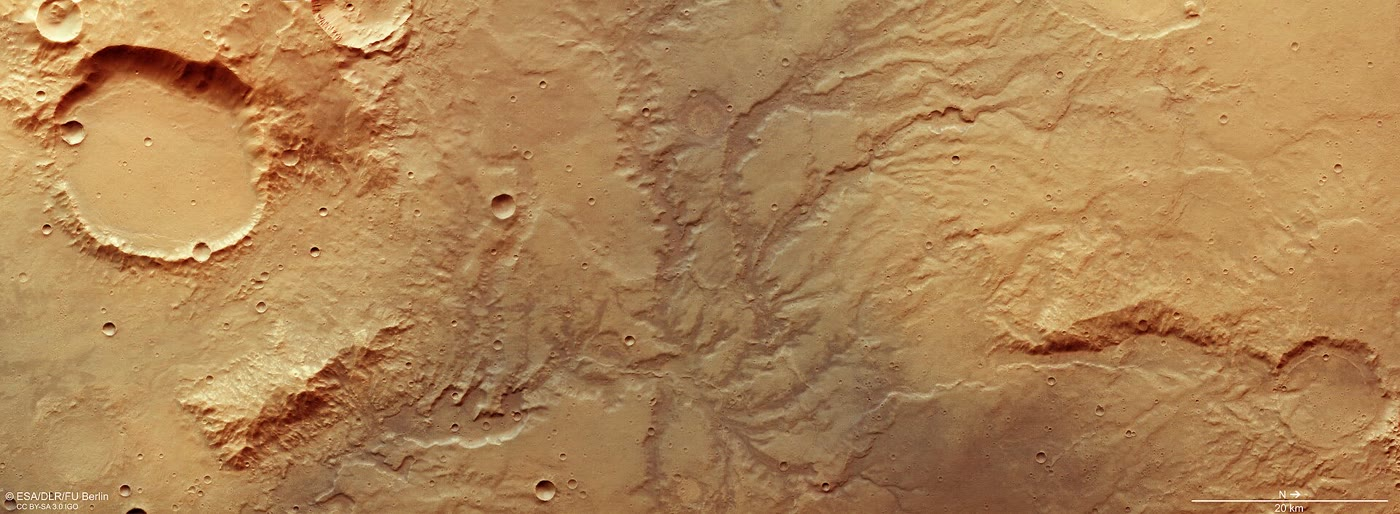
\includegraphics[width=\linewidth]{images/book5/b3-mars-valley-network.jpg}
\par\smallskip{\small Réseau de vallées asséchées sur Mars, photographié par la
caméra de Mars Express à environ \qty{14}{m} par pixel, près de \ang{17}\,S,
\ang{66}\,E~; le nord est à droite, et la barre d'échelle représente \qty{20}{km}.
Les affluents se rejoignent en aval dans des vallées plus grandes, dessin
d'un réseau de drainage. Image ESA/DLR/FU Berlin, CC BY-SA 3.0 IGO.}\label{fig:b3:planetary-atmospheres:valleys}
\end{omfigure}
% ledger: photo:b3-mars-valley-network

Les vallées et les chenaux d'écoulement de Mars supposent, selon les estimations géologiques,
une couche d'eau globale de 100 à \qty{1500}{m} d'épaisseur, contre 3 à
\qty{25}{m} dans sa glace et son air aujourd'hui. Une grande partie du reste s'est perdue dans
l'espace. L'orbiteur MAVEN a mesuré que le vent solaire arrache du gaz à Mars à raison d'environ
\qty{100}{g} par seconde, dont les trois quarts par la queue située derrière la planète, là où
s'écoule le vent solaire, et un quart dans un panache au-dessus des pôles~; lors des
tempêtes solaires de mars 2015, la perte s'est accélérée, et elle a probablement été bien plus
rapide lorsque le jeune Soleil était plus actif. Mars perd aussi de l'hydrogène, environ
\num{3e26} atomes par seconde en moyenne aujourd'hui~: maintenue pendant quatre
milliards d'années, cette perte ne représente qu'une couche d'eau globale
d'environ \qty{4}{m} d'épaisseur.
% ledger: gilli25:h-loss, lasp:maven

Le taux n'a pas toujours été celui d'aujourd'hui. L'obliquité de Mars, \ang{25.2}
aujourd'hui, a varié entre 0 et \ang{66} au cours des 250~Ma,
autour d'une moyenne proche de \ang{35}, tandis que celle de la Terre ne varie que
d'un peu plus d'un degré. Le mouvement est chaotique et ne peut pas être remonté sur
plusieurs milliards d'années~; des cratères elliptiques formés par des impacts rasants, dont l'orientation
garde la trace de l'obliquité, suggèrent une moyenne comprise entre environ 10 et \ang{30} au cours
des derniers 3.5~Ga environ. À forte obliquité, le pôle d'été se réchauffe,
davantage de vapeur d'eau s'élève, et les modèles climatiques font que la perte d'hydrogène
est vingt fois plus rapide~: sur l'histoire de Mars, cela représente une couche de l'ordre de
\qty{80}{m}.
% ledger: planet:Mars.obliq, gilli25:obliquity, holo18:obliquity, gilli25:h-loss

\section{Titan~: un cycle du méthane}\label{sec:b3:planetary-atmospheres:titan}

Titan, une lune plus petite que Mars, possède une atmosphère plus épaisse que celle de la Terre~:
une pression de surface supérieure d'environ 60\,\%, à \qty{-179}{\degreeCelsius}.
L'atmosphère est composée d'environ 95\,\% d'azote et de 5\,\% de méthane, et comme la
gravité de la lune est faible, elle s'étend dix fois plus haut que celle de la Terre, jusqu'à
près de \qty{600}{km}. Le rayonnement ultraviolet dissocie le méthane et l'azote
en haute altitude~; les fragments se recombinent en une brume orangée d'hydrocarbures plus lourds
qui masquent la surface à la lumière visible. Sous la brume, le méthane joue
le rôle de l'eau~: il se condense en nuages, il pleut, creuse des chenaux de rivières
et remplit des lacs et des mers de méthane et d'éthane.
% ledger: nasa:titan-surface, nasa:titan-facts

\begin{omfigure}
\centering
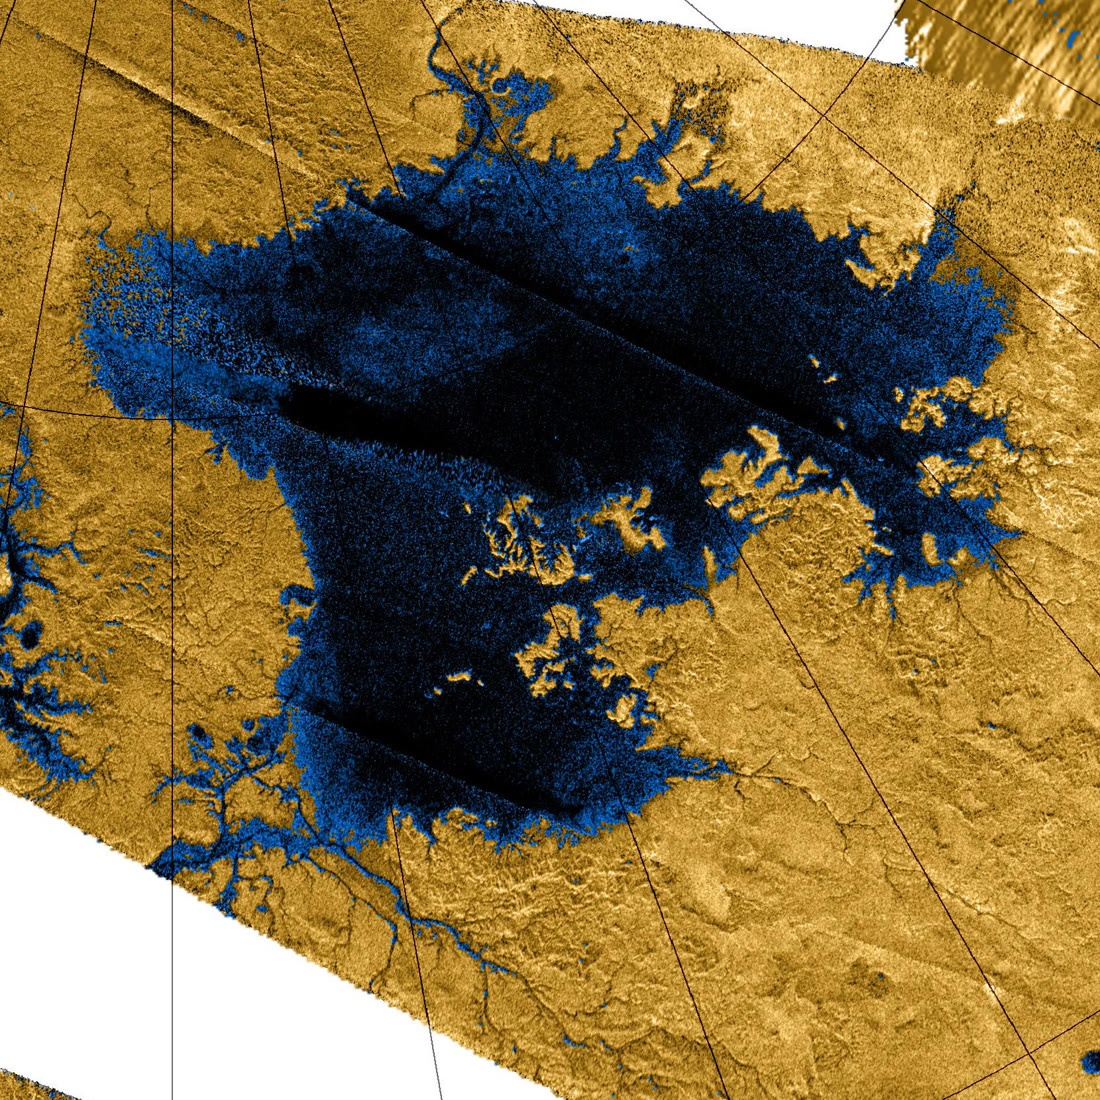
\includegraphics[width=0.5\linewidth]{images/book5/b3-ligeia-mare.jpg}
\par\smallskip{\small Ligeia Mare, une mer proche du pôle nord de Titan, en
mosaïque en fausses couleurs d'images radar de Cassini~: zones supposées liquides
en bleu et noir, sol solide teinté de brun, avec des baies et des îles
et des réseaux d'affluents présumés. Sur environ 400 lacs et mers de la partie nord
cartographiée, ceux dépassant \qty{26000}{km^2} concentrent 70\,\% de la surface.
NASA/JPL/USGS, domaine public.}\label{fig:b3:planetary-atmospheres:ligeia}
\end{omfigure}
% ledger: photo:b3-ligeia-mare

Qu'un liquide puisse se trouver à une surface dépend de son diagramme de phases et
de la pression et de la température qui y règnent. La surface de Titan se situe juste au-dessus du
point triple du méthane, \qty{90.67}{K} et \qty{0.117}{bar}, et en dessous de
son point critique~: du méthane liquide est possible, et du méthane à 5\,\% de
\qty{1.6}{bar} n'est pas loin de la saturation. La surface de Mars se situe près du
point triple de l'eau, celle de la Terre bien à l'intérieur de son domaine liquide, et
celle de Vénus au-dessus de la température critique de l'eau, \qty{647}{K}, où aucun
liquide ne peut exister.
% ledger: nist:methane-phase, iapws:triple-critical, nasa:titan-surface

\begin{omfigure}
\centering
\begin{tikzpicture}
\begin{axis}[width=0.8\linewidth, height=0.52\linewidth,
  xmin=60, xmax=800, ymin=1e-4, ymax=1000, ymode=log,
  xlabel={température (\unit{K})}, ylabel={pression (\unit{bar})},
  tick label style={font=\scriptsize}, label style={font=\small}]
\addplot[thick, omDef] table[x=T, y=p_bar] {figdata/out/bachelor-3-habitability-water.dat};
\addplot[thick, omDef, dashed] table[x=T, y=p_bar] {figdata/out/bachelor-3-habitability-ice.dat};
\addplot[thick, orange!80!black] table[x=T, y=p_bar] {figdata/out/bachelor-3-habitability-methane.dat};
\addplot[only marks, mark=*, mark size=1.6pt, omDef] coordinates {(273.16,0.00611657) (647.096,220.64)};
\addplot[only marks, mark=*, mark size=1.6pt, orange!80!black] coordinates {(90.67,0.1169) (190.6,46.1)};
\addplot[only marks, mark=square*, mark size=2.2pt, black] table[x=T, y=p_bar] {figdata/out/bachelor-3-habitability-bodies.dat};
\node[font=\scriptsize, anchor=south] at (axis cs:737,110) {Vénus};
\node[font=\scriptsize, anchor=west] at (axis cs:300,1.0) {Terre};
\node[font=\scriptsize, anchor=north] at (axis cs:214,0.0045) {Mars};
\node[font=\scriptsize, anchor=south] at (axis cs:94,2.2) {Titan};
\node[font=\scriptsize, omDef, anchor=west] at (axis cs:420,3) {eau~: liquide au-dessus, vapeur en dessous};
\node[font=\scriptsize, omDef, anchor=north west] at (axis cs:205,0.0012) {glace};
\node[font=\scriptsize, orange!80!black, anchor=west] at (axis cs:196,46) {méthane};
\node[font=\scriptsize, omDef, anchor=south east] at (axis cs:640,230) {point critique};
\end{axis}
\end{tikzpicture}
\par\smallskip{\small Les frontières entre la vapeur et l'eau condensée
(bleu~: liquide--vapeur, du point triple au point critique~;
en tirets~: glace--vapeur) et entre méthane liquide et sa vapeur (orange),
avec les états moyens de surface de Vénus, de la Terre, de Mars et de Titan
(carrés). Un liquide peut se trouver sur une surface dont la pression est située au-dessus de la
courbe de ce liquide, entre ses températures
triple et critique.}\label{fig:b3:planetary-atmospheres:phases}
\end{omfigure}
% ledger: iapws:vapour-pressure, iapws4:sublimation, iapws:triple-critical, nist:methane-phase, nasa:venus-atm, planet:Earth.Tmean, planet:Earth.psurf, nasa:mars-atm, nasa:titan-surface

Titan retient facilement son azote~: à son \omterm{def:b3:planetary-atmospheres:exobase}{exobase} $\lambda = 41$ pour
l'azote. Son hydrogène, avec $\lambda$ voisin de 1.5, s'échappe presque librement, et
l'échappement de l'hydrogène moléculaire est fixé plus bas par le flux limité
traversant l'\omterm{def:b3:planetary-atmospheres:hydrodynamic}{homopause}, comme sur la Terre. Les composés lourds formés à partir du
méthane dissocié se déposent à la surface, où ils constituent le sable de vastes
champs de dunes.
% ledger: gronoff:jeans-table, gronoff:diffusion, nasa:titan-surface

\section{Habitabilité planétaire}\label{sec:b3:planetary-atmospheres:habitability}

La zone habitable des manuels scolaires est l'intervalle des distances à une
étoile à laquelle une planète semblable à la Terre peut conserver de l'eau liquide à
sa surface. Ses bords sont les limites rencontrées dans ce chapitre.

\begin{definition}[Habitabilité planétaire]\label{def:b3:planetary-atmospheres:habitability}
L'\emph{habitabilité planétaire}\index{habitabilité planétaire} d'une
planète est sa capacité à conserver de l'eau liquide à sa surface sur des
échelles de temps géologiques~: elle reçoit un flux stellaire compris dans les
limites de la zone habitable, elle retient son atmosphère et son eau face à
l'échappement, et un cycle long du carbone régule son climat.
\end{definition}

Le bord interne de la zone habitable est fixé par l'\omterm{def:b3:planetary-atmospheres:runaway}{effet de serre humide} ou par
l'\omterm{def:b3:planetary-atmospheres:runaway}{effet de serre galopant}~: une planète de type terrestre autour du Soleil devient humide à
\qty{0.99}{au} et s'emballe à \qty{0.97}{au}. Le bord externe est le
\emph{effet de serre maximal}~: l'ajout de dioxyde de carbone ne réchauffe une planète que jusqu'à ce que le gaz
supplémentaire renvoie vers l'espace davantage de lumière solaire que son effet de serre n'en gagne~;
autour du Soleil, cela se produit à
\qty{1.70}{au}, sous environ \qty{8}{bar} de dioxyde de carbone. Ce sont des bords
conservatifs, calculés sans nuages. Deux bords empiriques sont plus larges~:
Vénus semble n'avoir eu aucune eau de surface pendant au moins 1~Ga,
alors qu'elle recevait 1.76 fois l'ensoleillement actuel de la Terre (\qty{0.75}{au})~;
Mars a connu de l'eau courante lorsqu'elle recevait 0.32 fois cet ensoleillement, si ses
vallées sont vieilles de 3.8~Ga (\qty{1.77}{au}). Autour d'étoiles plus froides, ces mêmes limites
se situent à des flux plus faibles, car leur lumière plus rouge est moins diffusée et
davantage absorbée par l'eau et le dioxyde de carbone.
% ledger: kopparapu13:runaway, kopparapu13:outer, kopparapu13:hz-fit

\begin{omfigure}
\centering
\begin{tikzpicture}
\begin{axis}[width=0.8\linewidth, height=0.5\linewidth,
  xmin=0, xmax=2.1, ymin=2600, ymax=7200, x dir=reverse,
  xlabel={flux stellaire reçu / Terre actuelle},
  ylabel={température stellaire (\unit{K})},
  tick label style={font=\scriptsize}, label style={font=\small},
  legend style={font=\scriptsize, at={(0.5,-0.24)}, anchor=north, legend columns=2, draw=none}]
\addplot[name path=mg, thick, omDef] table[x=mg, y=Teff] {figdata/out/bachelor-3-habitability-hz.dat};
\addlegendentry{effet de serre humide}
\addplot[name path=maxg, thick, red!70!black] table[x=maxg, y=Teff] {figdata/out/bachelor-3-habitability-hz.dat};
\addlegendentry{effet de serre maximal}
\addplot[thin, omDef, dashed] table[x=rg, y=Teff] {figdata/out/bachelor-3-habitability-hz.dat};
\addlegendentry{effet de serre galopant}
\addplot[thin, black!60, densely dotted] table[x=rv, y=Teff] {figdata/out/bachelor-3-habitability-hz.dat};
\addlegendentry{Vénus récente, Mars primitive}
\addplot[thin, black!60, densely dotted, forget plot] table[x=em, y=Teff] {figdata/out/bachelor-3-habitability-hz.dat};
\addplot[green!30, opacity=0.5, forget plot] fill between[of=mg and maxg];
\addplot[only marks, mark=*, mark size=2pt, black, forget plot] coordinates {(1.911,5780) (1.0,5780) (0.431,5780)};
\node[font=\scriptsize, anchor=south] at (axis cs:1.911,5800) {Vénus};
\node[font=\scriptsize, anchor=west, xshift=2pt] at (axis cs:1.0,5780) {Terre};
\node[font=\scriptsize, anchor=east, xshift=-2pt] at (axis cs:0.431,5780) {Mars};
\end{axis}
\end{tikzpicture}
\par\smallskip{\small La zone habitable d'une planète semblable à la Terre, selon
le flux stellaire qu'elle reçoit en fonction de la température de son étoile (en grisé~:
entre l'\omterm{def:b3:planetary-atmospheres:runaway}{effet de serre humide} et l'effet de serre maximal). En pointillés~: les
limites empiriques tirées de Vénus récente et de Mars primitive. Les ajustements
sont ceux d'un modèle climatique sans nuages, valables de 2600 à
\qty{7200}{K}.}\label{fig:b3:planetary-atmospheres:hz}
\end{omfigure}
% ledger: kopparapu13:hz-fit, nasa:venus, nasa:mars

La distance ne suffit pas. Une planète doit retenir son atmosphère~: une planète
petite ou chaude, dont le \omterm{def:b3:planetary-atmospheres:jeans-escape}{paramètre d'échappement} est faible, perd son hydrogène
et, avec lui, son eau, tandis qu'une planète en \omterm{def:b3:planetary-atmospheres:runaway}{effet de serre humide} s'assèche
par le haut. Il lui faut aussi maintenir son climat stable pendant des milliards
d'années, alors que son étoile s'éclaircit~: sur la Terre, le thermostat de
l'altération des silicates, au cœur du cycle long du carbone, fait baisser le
dioxyde de carbone lorsque le climat se réchauffe et le laisse s'accumuler lorsqu'il
se refroidit. Sur Vénus, sans tectonique des plaques, le dioxyde de carbone dégazé
n'a aucun moyen de retourner dans les roches et s'est accumulé dans l'air~; il
en contient aujourd'hui à peu près autant que la Terre en a piégé dans les roches
carbonatées. Le fait qu'un champ magnétique protège une atmosphère fait débat~: il
la met à l'abri du vent solaire dans sa partie haute, mais il ouvre aussi d'autres
voies d'échappement, comme l'écoulement d'ions près des pôles, et l'habitabilité
d'une planète ne se lit pas dans sa seule position au sein de la zone habitable.
% ledger: arney18:venus-loss, gronoff21:magnetic, gronoff:nonthermal

\section{Exercices}

\begin{exercise}[$\star$]\label{exo:b3:planetary-atmospheres:1}
Calculer la hauteur d'échelle $H = RT/Mg$ près de la surface de Vénus
(\qty{737}{K}, dioxyde de carbone de masse molaire \qty{44.01}{g.mol^{-1}},
$g = \qty{8.87}{m.s^{-2}}$), de la Terre (\qty{288}{K},
\qty{28.97}{g.mol^{-1}}, \qty{9.80}{m.s^{-2}}), de Mars (\qty{214}{K},
\qty{43.34}{g.mol^{-1}}, \qty{3.71}{m.s^{-2}}) et de Titan (\qty{94}{K},
\qty{28.0}{g.mol^{-1}}, \qty{1.35}{m.s^{-2}}). Quelle atmosphère est la
plus étendue, et pourquoi~?
\end{exercise}

\begin{exercise}[$\star$]\label{exo:b3:planetary-atmospheres:2}
L'\omterm{def:b3:planetary-atmospheres:exobase}{exobase} de la Terre se situe à \qty{500}{km} (rayon \qty{6878}{km})~; sa
température varie de 800 à \qty{1600}{K} au cours du cycle solaire. Prendre la
masse de la Terre égale à \qty{5.97e24}{kg}. Calculer le \omterm{def:b3:planetary-atmospheres:jeans-escape}{paramètre d'échappement}
des atomes d'hydrogène aux deux températures, ainsi que la fraction
qui s'échappe $(1 + \lambda)e^{-\lambda}$. De quel facteur le cycle solaire la modifie-t-il~?
\end{exercise}

\begin{exercise}[$\star$]\label{exo:b3:planetary-atmospheres:3}
Autour du Soleil, une planète semblable à la Terre devient humide au flux $S_\mathrm{eff}
= 1.014$, s'emballe à 1.0512 et atteint l'effet de serre maximal à 0.3438
(flux relatifs à celui de la Terre). (a)~Calculer les trois distances, en
unités astronomiques. (b)~Vénus et Mars reçoivent respectivement 1.91 et 0.43 fois
la lumière solaire de la Terre. Les placer.
\end{exercise}

\begin{exercise}[$\star$]\label{exo:b3:planetary-atmospheres:4}
La pression de vapeur du méthane liquide vaut $\log_{10}(p/\unit{bar}) = 3.9895 -
443.028/(T/\unit{K} - 0.49)$. (a)~La calculer à la surface de Titan,
\qty{94.15}{K}. (b)~Le méthane forme 5\,\% de l'air de Titan à \qty{1.6}{bar}.
Calculer sa pression partielle et son humidité relative. (c)~Que suggère le
résultat quant à l'évaporation des mers de Titan~?
\end{exercise}

\begin{exercise}[$\star\star$]\label{exo:b3:planetary-atmospheres:5}
À l'\omterm{def:b3:planetary-atmospheres:exobase}{exobase} de la Terre (\qty{1000}{K}, $\lambda = 7.02$ pour l'hydrogène),
calculer le \omterm{def:b3:planetary-atmospheres:jeans-escape}{paramètre d'échappement} du deutérium, sa vitesse thermique relative à
celle de l'hydrogène et le rapport des flux de Jeans par atome, D sur H. L'\omterm{def:b3:planetary-atmospheres:jeans-escape}{échappement
de Jeans} est-il un filtre isotopique puissant~?
\end{exercise}

\begin{exercise}[$\star\star$]\label{exo:b3:planetary-atmospheres:6}
Le rapport D/H de l'eau de Vénus vaut \num{0.016}~; celui de l'eau de mer sur
la Terre vaut \num{1.5575e-4}. (a)~Calculer l'enrichissement. (b)~En l'absence
totale d'échappement du deutérium, quel est le plus petit inventaire passé d'eau
de Vénus, sachant qu'il en reste \qty{6e15}{kg} aujourd'hui~? Quelle profondeur
formerait-il réparti sur la surface de la planète, \qty{4.60e14}{m^2}~? (c)~Quelle
diminution du réservoir exigerait un \omterm{def:b3:planetary-atmospheres:hydrodynamic}{échappement limité par la diffusion}, avec $\alpha = 0.8$~? Conclure.
\end{exercise}

\begin{exercise}[$\star\star$]\label{exo:b3:planetary-atmospheres:7}
Mars, de rayon \qty{3389.5}{km}, perd environ \num{3e26} atomes d'hydrogène
par seconde. (a)~Si chaque paire d'atomes provient d'une molécule d'eau, quelle
couche d'eau globale la perte retire-t-elle en quatre milliards d'années~?
(b)~Même question à \num{6e27} atomes par seconde, le taux d'une forte
obliquité. (c)~Comparer avec les \qty{100}{m} à \qty{1500}{m} qu'exigent les
vallées et les chenaux.
\end{exercise}

\begin{exercise}[$\star\star$]\label{exo:b3:planetary-atmospheres:8}
(a)~Calculer la masse de l'atmosphère de Mars à partir de sa pression
moyenne en surface, \qty{636}{Pa}, de sa gravité, \qty{3.71}{m.s^{-2}}, et de son
rayon. (b)~Le vent solaire arrache environ \qty{100}{g} de gaz par seconde.
Quelle masse cela retire-t-il en quatre milliards d'années, et en combien de temps
elle retirerait l'atmosphère actuelle~? (c)~Pourquoi est-ce une sous-estimation de la
perte passée~?
\end{exercise}

\begin{exercise}[$\star\star$]\label{exo:b3:planetary-atmospheres:9}
Une planète de type terrestre, dotée d'une atmosphère de vapeur sans nuages, réfléchit 19.3\,\%
de la lumière solaire qu'elle reçoit~; son rayonnement infrarouge ne peut dépasser
\qty{291}{W.m^{-2}}. (a)~Au-dessus de quel flux solaire, en watts par mètre carré
et rapporté à celui de la Terre, \qty{1361}{W.m^{-2}}, s'emballe-t-elle~?
(b)~Comparer avec Vénus aujourd'hui, \qty{2601}{W.m^{-2}}, et avec une jeune Vénus
sous un Soleil à 70\,\% de sa luminosité actuelle. (c)~Pourquoi la
conclusion pour la jeune Vénus n'est-elle pas définitive~?
\end{exercise}

\begin{exercise}[$\star\star\star$]\label{exo:b3:planetary-atmospheres:10}
Une thermosphère modèle d'oxygène atomique est isotherme à \qty{1000}{K}, avec
$n = \qty{1e16}{m^{-3}}$ à \qty{200}{km}~; prendre $g =
\qty{9.21}{m.s^{-2}}$ à cette altitude et une section efficace de collision
$\sigma_c = \qty{3e-19}{m^2}$. (a)~Calculer la hauteur d'échelle de l'oxygène.
(b)~Calculer la densité à l'\omterm{def:b3:planetary-atmospheres:exobase}{exobase} et la hauteur de l'\omterm{def:b3:planetary-atmospheres:exobase}{exobase}.
(c)~La gravité diminue avec l'altitude. Cela déplace-t-il l'\omterm{def:b3:planetary-atmospheres:exobase}{exobase} vers le haut ou
vers le bas~?
\end{exercise}

\begin{exercise}[$\star\star\star$]\label{exo:b3:planetary-atmospheres:11}
(a)~Supposons que la stratosphère terrestre devienne humide, avec un rapport de mélange
de vapeur d'eau de \num{3e-3} (compté comme $\ce{H2}$). Avec la limite
de diffusion $\num{3.0e13}\,f$ molécules de $\ce{H2}$ par centimètre carré et
par seconde, à \qty{200}{K}, calculer la perte d'hydrogène de la Terre
entière (rayon \qty{6371}{km}). (b)~En combien de temps un océan,
soit \qty{1.4e24}{g} d'eau, serait-il épuisé~? Comparer avec l'âge de la Terre.
\end{exercise}

\begin{exercise}[$\star\star\star$]\label{exo:b3:planetary-atmospheres:12}
Dans une haute atmosphère de vapeur pure, absorbant comme un gaz gris, avec $\kappa =
\qty{0.005}{m^2.kg^{-1}}$, sur une planète de $g = \qty{9.81}{m.s^{-2}}$
et $D = 1.66$~: (a)~calculer la pression $p_1$ du niveau rayonnant~;
(b)~avec $p_\mathrm{sat}(T) = \qty{611.657}{Pa}\,\exp[(L/R_v)(1/T_t -
1/T)]$, $L = \qty{2.5e6}{J.kg^{-1}}$, $R_v = \qty{461.5}{J.kg^{-1}.K^{-1}}$,
$T_t = \qty{273.16}{K}$, calculer sa température et la limite de rayonnement.
(c)~La limite raie par raie est \qty{291}{W.m^{-2}}. Le
$\kappa$ effectif de la vapeur d'eau réelle doit-il être plus grand ou plus petit~?
\end{exercise}

\section{Problème~: Kepos gardera-t-elle son eau~?}

\begin{problem}[{Problème du week-end --- échappement et habitabilité de la
planète océanique inventée}]
\label{pb:b3:planetary-atmospheres:1}
Kepos est une planète inventée de masse \qty{5.2e24}{kg} et de rayon
\qty{6200}{km}, pourvue d'océans et d'une atmosphère d'azote et de dioxyde de carbone.
Elle orbite à \qty{0.60}{au} d'une étoile de luminosité 0.30 fois celle du
Soleil et de température effective \qty{4800}{K}. Son \omterm{def:b3:planetary-atmospheres:exobase}{exobase} se trouve à
\qty{500}{km} au-dessus de la surface, à \qty{1400}{K}, avec
\qty{2e11}{m^{-3}} atomes d'hydrogène~; son \omterm{def:b3:planetary-atmospheres:hydrodynamic}{homopause} est à \qty{200}{K},
où le dioxyde de carbone domine et où l'hydrogène sous toutes ses formes forme un
rapport de mélange $f = \num{1e-3}$, compté comme $\ce{H2}$. Un océan terrestre représente
\qty{1.4e24}{g} d'eau.

\medskip\noindent\textbf{Partie I --- L'exobase.}
\begin{enumerate}
\item Calculer la pesanteur de surface et la masse volumique moyenne de Kepos.
\item Calculer la vitesse de libération à l'\omterm{def:b3:planetary-atmospheres:exobase}{exobase}.
\item Calculer la vitesse thermique $u = \sqrt{2kT/m}$ de l'hydrogène, de l'hélium et
  de l'oxygène atomique à l'\omterm{def:b3:planetary-atmospheres:exobase}{exobase}.
\item Calculer leurs \omterm{def:b3:planetary-atmospheres:jeans-escape}{paramètres d'échappement}.
\item Lesquels d'entre eux peuvent s'échapper par \omterm{def:b3:planetary-atmospheres:jeans-escape}{échappement de Jeans} à un taux significatif~?
  L'un d'eux approche-t-il du régime hydrodynamique~?
\item Pendant une jeunesse active de son étoile, l'\omterm{def:b3:planetary-atmospheres:exobase}{exobase} de Kepos a pu
  atteindre \qty{3000}{K}. Quel était alors le \omterm{def:b3:planetary-atmospheres:jeans-escape}{paramètre d'échappement} de
  l'hydrogène, et que suggère-t-il~?
\end{enumerate}

\medskip\noindent\textbf{Partie II --- Échappement de Jeans de l'hydrogène.}
\begin{enumerate}[resume]
\item Calculer la fraction d'échappement $(1 + \lambda)e^{-\lambda}$ pour
  l'hydrogène.
\item Calculer le flux de Jeans de l'hydrogène, par mètre carré et par seconde.
\item Calculer le nombre d'atomes d'hydrogène qui quittent l'ensemble de
  l'\omterm{def:b3:planetary-atmospheres:exobase}{exobase} par seconde.
\item Combien d'atomes d'hydrogène contient un océan terrestre~?
\item À ce rythme, en combien de temps Kepos les perdrait-elle~?
\item Calculer le \omterm{def:b3:planetary-atmospheres:jeans-escape}{paramètre d'échappement} du deutérium et son efficacité
  d'échappement par rapport à l'hydrogène, par atome.
\end{enumerate}

\medskip\noindent\textbf{Partie III --- La limite de diffusion.}
\begin{enumerate}[resume]
\item Calculer la hauteur d'échelle du dioxyde de carbone à l'\omterm{def:b3:planetary-atmospheres:hydrodynamic}{homopause}.
\item Le paramètre de diffusion binaire de l'hydrogène dans le dioxyde de carbone est
  $b = \qty{1.2e19}{cm^{-1}.s^{-1}}$ à \qty{200}{K}. Calculer le
  flux limité par la diffusion de $\ce{H2}$, par mètre carré et par seconde.
\item Vérifier ce résultat par rapport à la limite terrestre, $\num{3.0e13}\,f$ molécules par
  centimètre carré et par seconde, ajustée à la gravité.
\item Calculer le nombre d'atomes d'hydrogène que la limite de diffusion peut
  fournir à la haute atmosphère de toute la planète par seconde (en prenant
  l'aire de la surface).
\item Comparer avec la question~9. Quel processus limite l'échappement, et que
  devient l'hydrogène de la thermosphère~?
\item Quelle densité d'hydrogène à l'\omterm{def:b3:planetary-atmospheres:exobase}{exobase} permettrait à l'\omterm{def:b3:planetary-atmospheres:jeans-escape}{échappement de Jeans}
  d'emporter tout cet apport~?
\item En combien de temps Kepos perdrait-elle un océan terrestre d'hydrogène
  au rythme limité par la diffusion~?
\end{enumerate}

\medskip\noindent\textbf{Partie IV --- Kepos est-elle dans la zone habitable~?}
\begin{enumerate}[resume]
\item Calculer le flux stellaire reçu par Kepos, par rapport à celui de la Terre.
\item Pour une étoile de \qty{4800}{K}, la limite de l'\omterm{def:b3:planetary-atmospheres:runaway}{effet de serre humide} se situe à
  $S_\mathrm{eff} = 0.939$, et la limite maximale de l'effet de serre à 0.290. Calculer les
  bornes de la zone habitable, en unités astronomiques, et placer Kepos.
\item De quel facteur l'étoile doit-elle gagner en luminosité avant que Kepos n'atteigne
  le bord intérieur de la zone~?
\item Avec un albédo de 0.3, calculer le rayonnement solaire que Kepos absorbe par
  mètre carré, et sa température d'équilibre. Comparer avec la \omterm{def:b3:planetary-atmospheres:runaway}{limite de
  l'effet de serre galopant}.
\item Si un climat plus chaud rendait humide la stratosphère de Kepos, avec
  $f = \num{3e-3}$, combien de temps durerait un océan terrestre~?
\item Donner le temps que met Kepos pour perdre un océan terrestre d'hydrogène par
  \omterm{def:b3:planetary-atmospheres:hydrodynamic}{échappement limité par la diffusion} avec $f = \num{1e-3}$, en milliards d'années, à
  deux chiffres significatifs.
\end{enumerate}
\end{problem}
% ledger: zahnle19:diffusion, kopparapu13:hz-fit, kopparapu13:runaway, gronoff:jeans, const:G, const:kB, const:NA
